\subsubsection{Explicación del problema}
El problema consiste en destruir a los androides del doctor Maki Gero mediante la menor cantidad posible de Kamehamehas lanzados por Goku.
A fin de resolver este problema modelamos a los androides como puntos en el plano y los Kamehameha como semirrectas en el mismo. Dicho es el problema se reduce a atravesar todos los puntos del plano con la menor cantidad de semirrectas.

Tenemos un plano infinito con N posiciones ocupadas. El problema consiste en remover dichos puntos dibujando semirrectas desde una posición inicial en una dirección indicada, los puntos que sean atravesados por la semirrecta se consideran removidos. La cantidad de semirrectas necesarias para remover todos los puntos debe ser la mínima posible.
Supongamos el siguiente plano con N = 3:

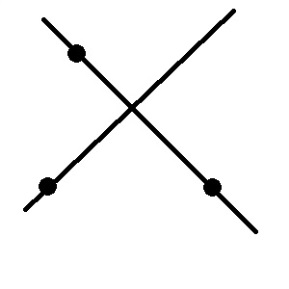
\includegraphics[width=\textwidth]{ex_ej_3}


Entonces se ve claramente que con dos rectas alcanza para solucionar el problema.






\subsubsection{Ideas e implementación}
Para resolver el problema usaremos la técnica de backtracking. Mediante el mismo iremos eligiendo de a 2 elementos dentro de un vector con las posiciones de los androides y calculando la pendiente de la recta que los une nos fijaremos si atraviesa posiciones de otros androides en su recorrido. Marcaremos todos estos puntos como androides destruidos.
Una posible solución es encontrada cuando no quedan androides por destruir.
La estructura del algoritmo de backtracking es la siguiente:

%//backtrack
%Voy iterando por cada enemigo aun vivo
%	tomo 2 enemigos aun vivos
%		"Dibujo" la recta por la cual pasan ambos enemigos
%		Marco como muertos, a todos los enemigos que esten en esa recta
%		llamo a backtrack //se vuelve a iterar sobre los enemigos q a partir de ese momento esten vivos y trazar nuevas rectas
%		marco como vivos, a todos los enemigos que hayan estado en esa recta ( por que asi, puedo considerar , en las proximas iteraciones, otras soluciones posibles)
%



\begin{algorithm}[h!]
\caption{Estructura del algoritmo de Backtracking}
\begin{algorithmic}[1]
	\Function{Backtrack}{}
	\If{no quedan mas androides por destruir}
		\State Mejor solución encontrada hasta ahora
		\State Guardo el vector de androides como mejor solución
	\Else
		\For{cada par de androides $a_1$, $a_2$}
            \If{$a_1$ y $a_2$ no estan destruidos}
                \If{la solución parcial es menor que la mejor solución +1}
                    \State Destruir los androides $a_1$, $a_2$
                    \State Destruir los androides en la semirrecta entre $a_1$ y $a_2$
                    \State Backtrack()
                    \State Restaurar los androides en la semirrecta entre $a_1$ y $a_2$
                    \State Restaurar los androides $a_1$, $a_2$                        
                \EndIf
            \EndIf
		\EndFor
	\EndIf
	\EndFunction
\end{algorithmic}
\end{algorithm}

\subsubsection{Podas}
En esta sección se explican las podas implementadas.

\begin{enumerate}
\item Una de las primeras podas que aplicamos es la de verificar si el androide no se encuentra ya destruido para no seguir por esa rama.
\item Aplicamos otra poda comparando que los 2 androides a unir con la semirecta no sean el mismo.
\item Aplicamos también una poda al comparar la solución parcial con la mejor solución encontrada hasta ese momento y solo seguimos en caso que sea posible mejorar la mejor solución encontrada hasta ese momento.
\end{enumerate}

